\chapter{Hiện thực hệ thống}
\label{chap:hien-thuc}

Chương này kể lại thiết kế ở chương~\ref{chap:thiet-ke} đã thành mã như thế nào. Lần lượt là công nghệ dùng, quy mô mã nguồn, vài đoạn mã tiêu biểu cho các mẫu thiết kế chính, giao diện người dùng và cấu hình triển khai.

\section{Công nghệ và quy mô mã nguồn}

Bảng~\ref{tab:cong-nghe} liệt kê công nghệ của từng thành phần. Toàn bộ mã nằm trong một monorepo, quản lý bằng pnpm và Turborepo, gồm ba gói: \code{apps/api}, \code{apps/web} và \code{packages/shared-types}. Gói cuối chứa kiểu dữ liệu và bảng quyền mà web và API cùng dùng, nhờ vậy hai bên không bao giờ hiểu một quyền theo hai cách khác nhau.

\begin{table}{Công nghệ sử dụng}
\label{tab:cong-nghe}
\small
\begin{tabularx}{\textwidth}{|P{3.4cm}|L|}
\hline
\textbf{Thành phần} & \textbf{Công nghệ} \\ \hline
Ngôn ngữ & TypeScript 5 cho API, web và các dự án sinh ra \\ \hline
API & NestJS 10, Socket.IO, Prisma 5, BullMQ 5, pdfkit, TypeScript compiler API \\ \hline
Cơ sở dữ liệu, hàng đợi & PostgreSQL 16 có pgvector, Redis 7 \\ \hline
Web & React 18, Vite 5, Ant Design 6 (antd 6.7, @ant-design/icons 6), Ant Design X cho Phòng họp, Ant Design Charts cho biểu đồ, TanStack Query, Zustand \\ \hline
Kiểm thử & Jest với ts-jest cho API, Vitest cho web, Playwright cho kiểm thử giao diện đầu cuối \\ \hline
LLM & Nhà cung cấp tương thích OpenAI (9Router, OpenAI, OpenRouter, Groq, DeepSeek, Gemini, Ollama) hoặc Anthropic, cấu hình trong ứng dụng, với \code{NINE_ROUTER_URL} là cổng mặc định \\ \hline
Triển khai & Docker (Node 20, nginx 1.27), Docker Compose \\ \hline
\end{tabularx}
\end{table}

Bảng~\ref{tab:quy-mo} cho biết quy mô mã nguồn lúc viết khoá luận, đếm tự động và không tính tệp kiểm thử. Phần web được đếm lại sau đợt nâng cấp Ant Design 6: số tệp tăng từ 76 lên 82 vì có thêm bốn tệp chủ đề và hai thành phần dùng chung, nhưng số dòng giảm từ 8\,715 xuống 8\,439 do nhiều đoạn tự dựng được thay bằng thành phần có sẵn. API gồm 26 mô-đun NestJS và 295 lớp được xuất ra (\code{export class}).

\begin{table}{Quy mô mã nguồn}
\label{tab:quy-mo}
\begin{tabular}{|l|r|r|}
\hline
\textbf{Phần} & \textbf{Số tệp} & \textbf{Số dòng} \\ \hline
API (\code{apps/api/src}) & 342 & 28\,753 \\ \hline
\quad trong đó tầng miền (\code{src/domain}) & 106 & 7\,226 \\ \hline
Web (\code{apps/web/src}) & 82 & 8\,439 \\ \hline
Bộ kiểm thử API (Jest) & 50 & không đếm \\ \hline
\end{tabular}
\end{table}

\section{Tầng miền}

Tầng miền chia thư mục theo khái niệm nghiệp vụ: \code{entities} (Project, Task, Milestone, Agent\ldots), \code{value-objects} (Money, ProjectStatus\ldots), \code{repositories} (chỉ có giao diện), \code{events} (sự kiện miền và \code{EventBus}), \code{agent} (máy trạng thái, bộ phát sự kiện, giao diện chiến lược, học), \code{workflow} (đồ thị, bộ giải phụ thuộc, phiên bản ngữ nghĩa, memento), cùng \code{security}, \code{audit}, \code{integration}, \code{reporting}, \code{analytics}, \code{estimation}, \code{quality}, \code{collaboration}.

Thực thể nào cũng tự giữ bất biến của mình. \code{Task.transitionTo} chỉ cho đi theo các bước hợp lệ: \code{todo} sang \code{in_progress}, sang \code{review}, sang \code{done}, và từ \code{review} quay về \code{in_progress} khi QA từ chối (Hình~\ref{fig:sm-cong-viec}). \code{Money} không nhận giá trị âm. Chính quy tắc này đã làm lộ ra một lỗi. \code{Task.getCostVariance()} ném ngoại lệ với mọi công việc chưa tiêu hết ngân sách, vì chênh lệch âm không biểu diễn được bằng \code{Money}. Hàm đã được sửa để trả về số đô-la có dấu.

\begin{figure}{Máy trạng thái của công việc}
\label{fig:sm-cong-viec}
\centering
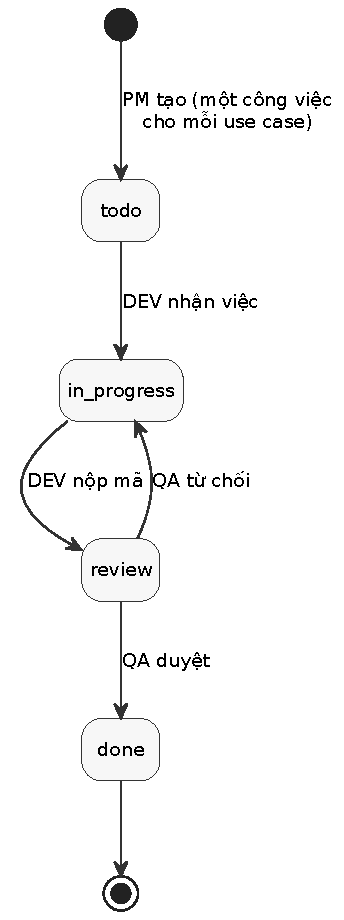
\includegraphics[height=0.32\textheight]{sodo/may-trang-thai-cong-viec.pdf}
\end{figure}

Đoạn mã~\ref{code:repo} là giao diện Repository của dự án. Giao diện nằm ở tầng miền và chỉ nhắc tới DTO của miền, không kiểu nào của Prisma lọt được vào đây.

\begin{codelisting}{Giao diện Repository của dự án ở tầng miền (rút gọn)}
\label{code:repo}
\begin{Verbatim}
// apps/api/src/domain/repositories/IProjectRepository.ts
export interface IProjectRepository {
  findById(id: string): Promise<ProjectDTO | null>;
  findAll(options?: {
    orderBy?: 'createdAt' | 'updatedAt';
    order?: 'asc' | 'desc';
  }): Promise<ProjectDTO[]>;
  create(data: CreateProjectData): Promise<ProjectDTO>;
  update(id: string, data: UpdateProjectData): Promise<ProjectDTO>;
}
\end{Verbatim}
\end{codelisting}

Lớp hiện thực \code{PrismaProjectRepository} nằm ở \code{src/infrastructure/persistence} và chỉ lấy những cột mà DTO cần. Chi tiết này nghe thì nhỏ nhưng đo được hẳn hoi. Kiểm thử tải cho thấy truy vấn danh sách dự án từng kéo về cả ngữ cảnh JSON của lượt chạy mới nhất rồi bỏ đi. Sửa xong, thời gian truy vấn giảm từ 46~ms xuống 9~ms.

\section{Tác tử}

Đoạn mã~\ref{code:base-agent} là phần lõi của \code{BaseAgent.execute()}. Mỗi lần gọi tạo một máy trạng thái riêng, hai bước \code{think} và \code{act} được uỷ cho chiến lược, còn việc phát sự kiện, chuyển trạng thái và dọn dẹp do lớp cơ sở lo.

\begin{codelisting}{Khung thuật toán của tác tử trong BaseAgent (rút gọn)}
\label{code:base-agent}
\begin{Verbatim}
// apps/api/src/modules/agents/base.agent.ts
async execute(input: AgentContext): Promise<AgentResult<TOutput>> {
  const context = this.prepareContext(input);     // theo RoleProfile
  const lifecycle = new AgentStateMachine(AgentState.IDLE);
  this.running.add(lifecycle);                     // mỗi lần chạy một máy
  try {
    await this.publish(new TaskAssignedEvent(/* ... */));
    this.transition(lifecycle, AgentState.THINKING, 'Starting');
    const thought = await this.thinkingStrategy.think(context);
    this.transition(lifecycle, AgentState.ACTING, 'Executing');
    const action = await this.actionStrategy.act(context, thought);
    this.transition(lifecycle, AgentState.COMPLETED, 'Done');
    // lưu ký ức, phát AgentCompletedTaskEvent, quay về IDLE ...
  } catch (error) {
    this.transition(lifecycle, AgentState.ERROR, (error as Error).message);
    // ...
  } finally {
    this.running.delete(lifecycle);
  }
}
\end{Verbatim}
\end{codelisting}

Mỗi vai trò có một tệp hồ sơ trong \code{modules/agents/profiles} và hai chiến lược trong \code{modules/agents/strategies}. NestJS tiêm danh sách tác tử vào qua token \code{AGENTS}, rồi \code{AgentOrchestrator} dựng bảng tra theo vai trò và báo lỗi ngay nếu có hai tác tử trùng vai trò. Muốn thêm vai trò thứ chín, người phát triển thêm một giá trị \code{AgentRole}, một hồ sơ, hai chiến lược và một dòng đăng ký provider. Bộ điều phối và bộ máy quy trình giữ nguyên.

Chiến lược hành động của BA, Architect, DEV và QC ghi sản phẩm qua \code{ProjectWorkspace}. \code{OoadArtifactService}, một Facade, dựng tài liệu và khung mã từ mẫu Handlebars. Nội dung LLM trả về được tách thành các khối \code{<CODE filepath="...">}, và từng đường dẫn được kiểm tra trước khi ghi.

Đoạn mã~\ref{code:decorator} là Decorator ghi chi phí. Lớp này hiện thực đúng giao diện \code{ILLMProvider} mà nó bọc, nên chiến lược tác tử không phân biệt được mình đang gọi nhà cung cấp gốc hay bản đã bọc. Nếu việc ghi nhật ký bị lỗi thì lời gọi chính vẫn chạy bình thường, chỉ có thêm một cảnh báo.

\begin{codelisting}{Decorator ghi chi phí lời gọi LLM (rút gọn)}
\label{code:decorator}
\begin{Verbatim}
// apps/api/src/modules/llm/usage-tracking.provider.ts
export class UsageTrackingLLMProvider implements ILLMProvider {
  constructor(
    private readonly inner: ILLMProvider,
    private readonly apiUsageService: ApiUsageService,
    private readonly usage: UsageContext,
  ) {}

  async chat(params: ChatParams): Promise<ChatResult> {
    const startTime = Date.now();
    const result = await this.inner.chat(params);
    await this.apiUsageService.logUsage({
      projectId: this.usage.projectId,
      agentRole: this.usage.agentRole,
      requestedModel: params.model,
      promptTokens: result.tokenUsage?.promptTokens ?? 0,
      completionTokens: result.tokenUsage?.completionTokens ?? 0,
      responseTimeMs: Date.now() - startTime,
      // ...
    }).catch(err => this.logger.warn(/* ... */));
    return result;
  }
}
\end{Verbatim}
\end{codelisting}

\section{Bộ máy quy trình}

\code{WorkflowEngine} giữ một bảng ánh xạ từ loại nút sang \code{NodeExecutionStrategy}. Giao diện chiến lược rất nhỏ, như Đoạn mã~\ref{code:node}: một thuộc tính cho biết loại nút và một phương thức thực thi.

\begin{codelisting}{Giao diện chiến lược thực thi nút}
\label{code:node}
\begin{Verbatim}
// apps/api/src/modules/workflow/strategies/node-execution-strategy.ts
export interface NodeExecutionStrategy {
  readonly type: NodeType;
  execute(node: WorkflowNode, run: WorkflowRunRecord,
          ctx: NodeExecutionContext): Promise<NodeResult>;
}
\end{Verbatim}
\end{codelisting}

Có bảy lớp hiện thực giao diện này: \code{AgentTaskStrategy}, \code{SubWorkflowStrategy}, \code{QualityGateStrategy}, \code{ConditionStrategy}, \code{ParallelStrategy}, \code{HumanApprovalStrategy} và \code{AgentCollaborationStrategy}. Khi có Redis, mỗi nút là một công việc BullMQ, tối đa 5 công việc chạy cùng lúc. Không có Redis thì nút chạy trực tiếp. Nút nào xong thì \code{handleJobCompletion} ghi bước kèm thời lượng, chụp memento và chọn cạnh kế tiếp. Nút vẫn lỗi sau các lần thử lại thì kết quả được đổi thành \code{failure}, để lượt chạy đi theo cạnh \code{onFail} hoặc dừng ở trạng thái \code{failed}.

Mẫu quy trình là lớp con của \code{WorkflowTemplate}, có danh sách tham số định kiểu (số, chuỗi, enum, boolean) được kiểm tra trước khi dựng định nghĩa quy trình. Ví dụ mẫu \textit{REST API backend} có tham số \code{database} kiểu enum. Giá trị này được đưa vào lời nhắc thiết kế của Architect như một ràng buộc của nút, để Repository được thiết kế đúng cho loại cơ sở dữ liệu đã chọn. Hình~\ref{fig:template-form} là phần cuối của hộp thoại tạo dự án. Các ô tham số được sinh ra từ danh sách tham số của mẫu, bên dưới có bản xem trước đồ thị quy trình kèm mã phiên bản.

\begin{figure}{Biểu mẫu tham số của mẫu quy trình}
\label{fig:template-form}
\centering
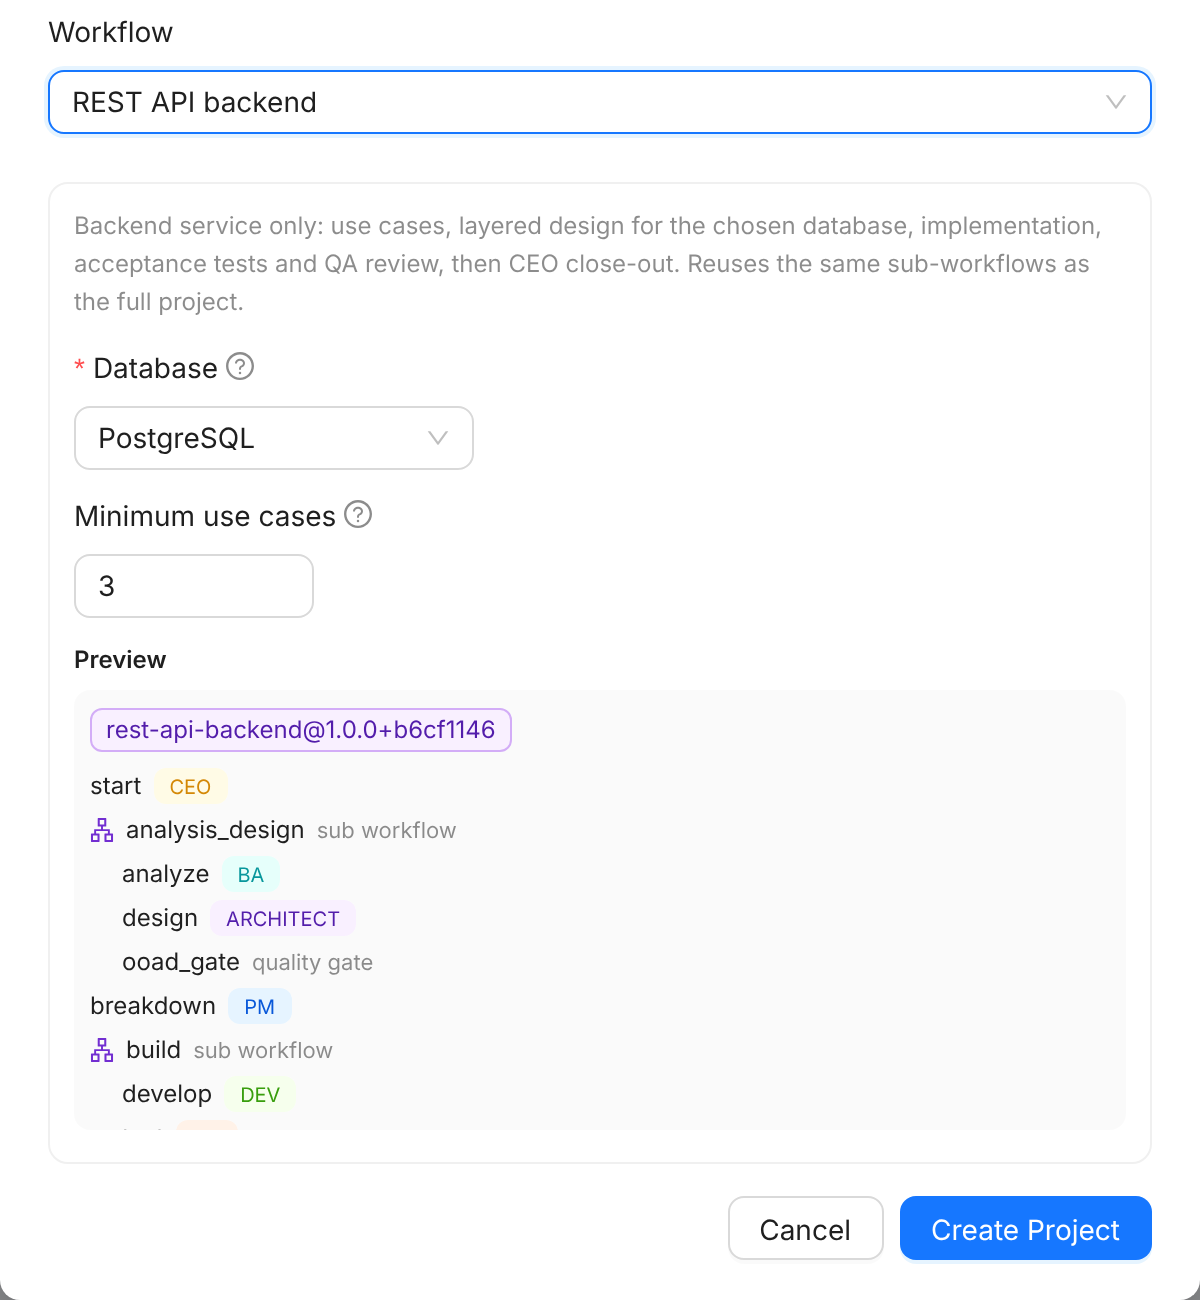
\includegraphics[width=0.5\textwidth]{anh/template-form.png}
\end{figure}

\section{Tính năng doanh nghiệp}

\begin{itemize}
\item \textbf{Phân quyền.} Controller gắn decorator \code{@RequirePermission} với tham số như \code{Permission.PROJECT_CREATE}, còn quyền của từng vai trò lấy từ gói \code{shared-types}. Giao diện giấu những nút mà người dùng không có quyền bấm, như nút \textit{New Project} với người xem, nhưng API vẫn tự kiểm tra quyền chứ không trông vào giao diện.
\item \textbf{Kiểm toán.} Route gắn \texttt{@Audited(\{ action: 'approval.approve', resourceType: 'Approval', idParam: 'id' \})}, và interceptor ghi kết quả \textit{ok} hoặc \textit{denied} kèm địa chỉ IP. Trang nhật ký có bộ lọc, phân trang và nút xuất CSV. Ô nào bắt đầu bằng \code{=}, \code{+}, \code{-}, \code{@} được thoát để chống chèn công thức khi mở bằng bảng tính. Trong Hình~\ref{fig:audit} có thể thấy ba loại tác nhân nằm chung một bảng: người dùng (đăng nhập, duyệt), tác tử (hoàn thành công việc) và hệ thống (kết thúc lượt chạy).
\item \textbf{Xuất báo cáo.} Hỗ trợ JSON, CSV và PDF. PDF dựng bằng pdfkit với phông chữ có dấu tiếng Việt. Báo cáo tuần được ghi vào thư mục \code{reports/} của dự án thay vì gửi email.
\item \textbf{Nhà cung cấp LLM.} Trang \textit{LLM Providers}, chỉ dành cho quản trị viên, cho phép thêm nhà cung cấp từ mẫu có sẵn, kiểm tra kết nối, lấy danh sách mô hình hoặc thêm mô hình theo mã (Hình~\ref{fig:providers}). Ở trang \textit{Agent Models}, quản trị viên chọn mô hình cho từng vai trò từ danh sách nhóm theo nhà cung cấp. Mọi thay đổi đều được ghi kiểm toán với khoá đã che.
\item \textbf{Điều khiển lượt chạy.} Đầu trang chi tiết dự án có nút tạm dừng, tiếp tục, huỷ, bắt đầu quy trình và chỉnh ngân sách. Một biểu ngữ báo khi ngân sách đã hết hoặc quy trình chưa bắt đầu. Phê duyệt được trả lời trong một hộp thoại có tóm tắt dễ đọc, và ai từ chối thì phải ghi lý do.
\end{itemize}

\begin{figure}{Trang nhật ký kiểm toán}
\label{fig:audit}
\centering
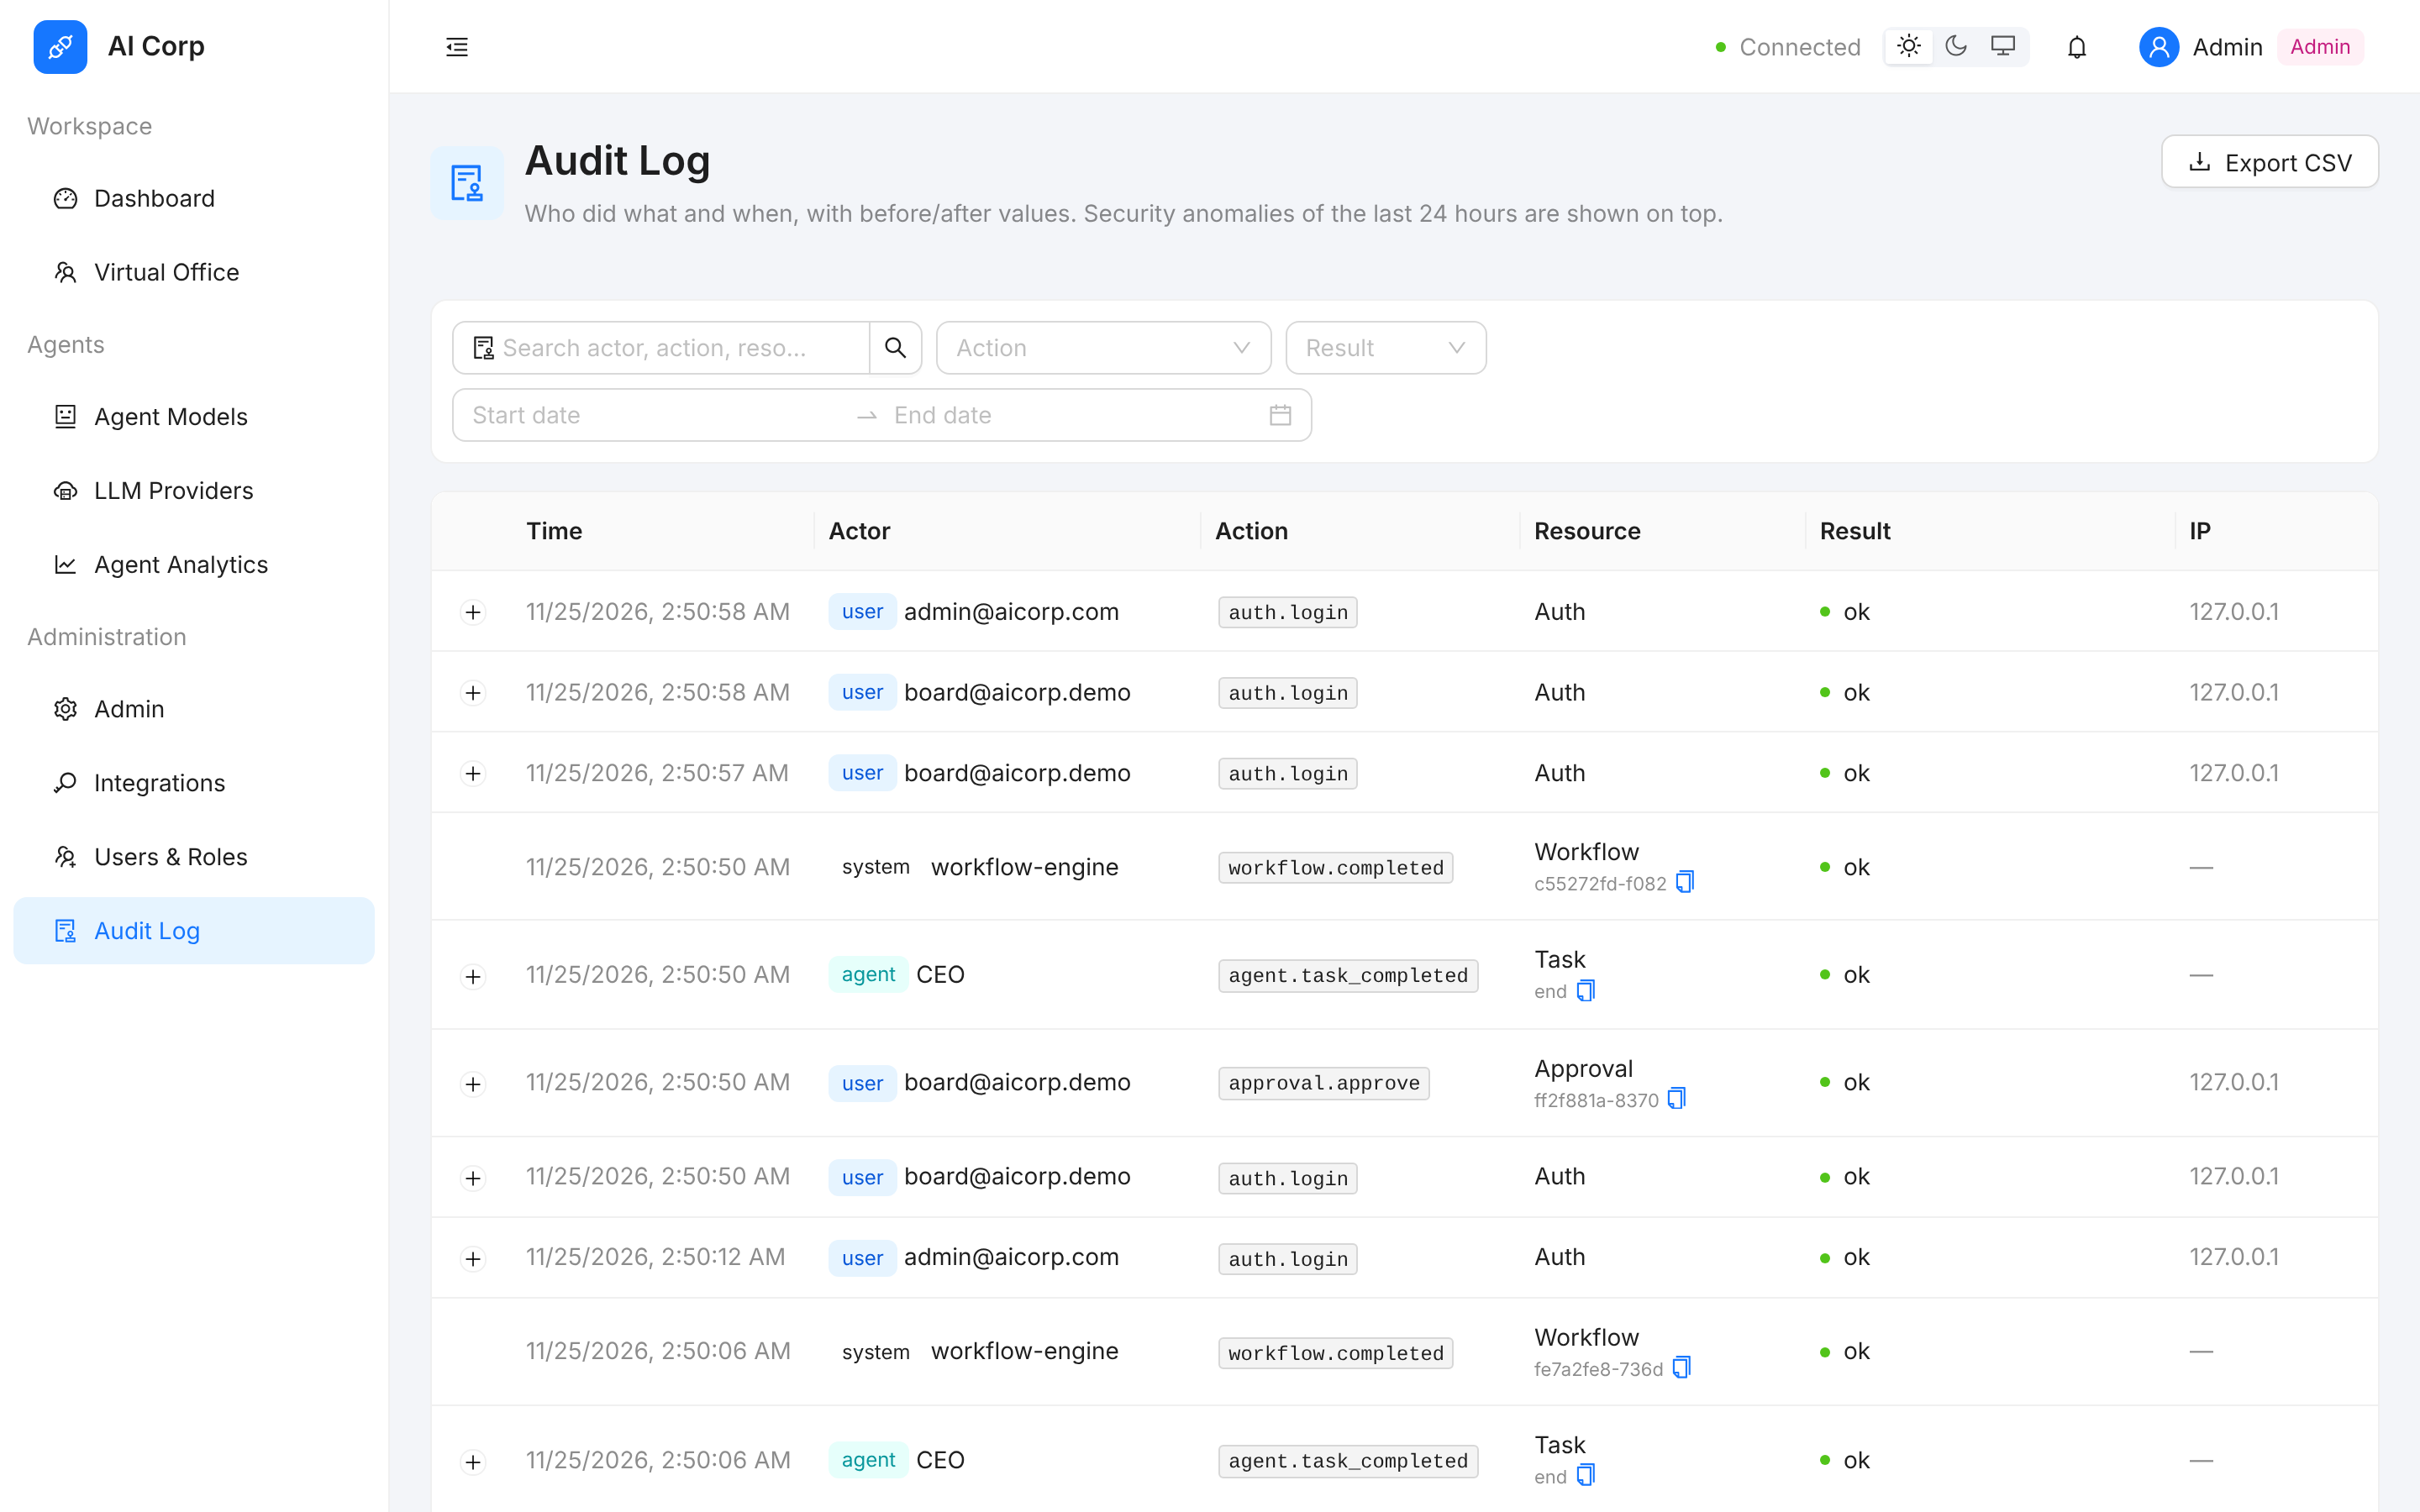
\includegraphics[width=\textwidth]{anh/audit-log.png}
\end{figure}

\begin{figure}{Trang quản lý nhà cung cấp LLM}
\label{fig:providers}
\centering
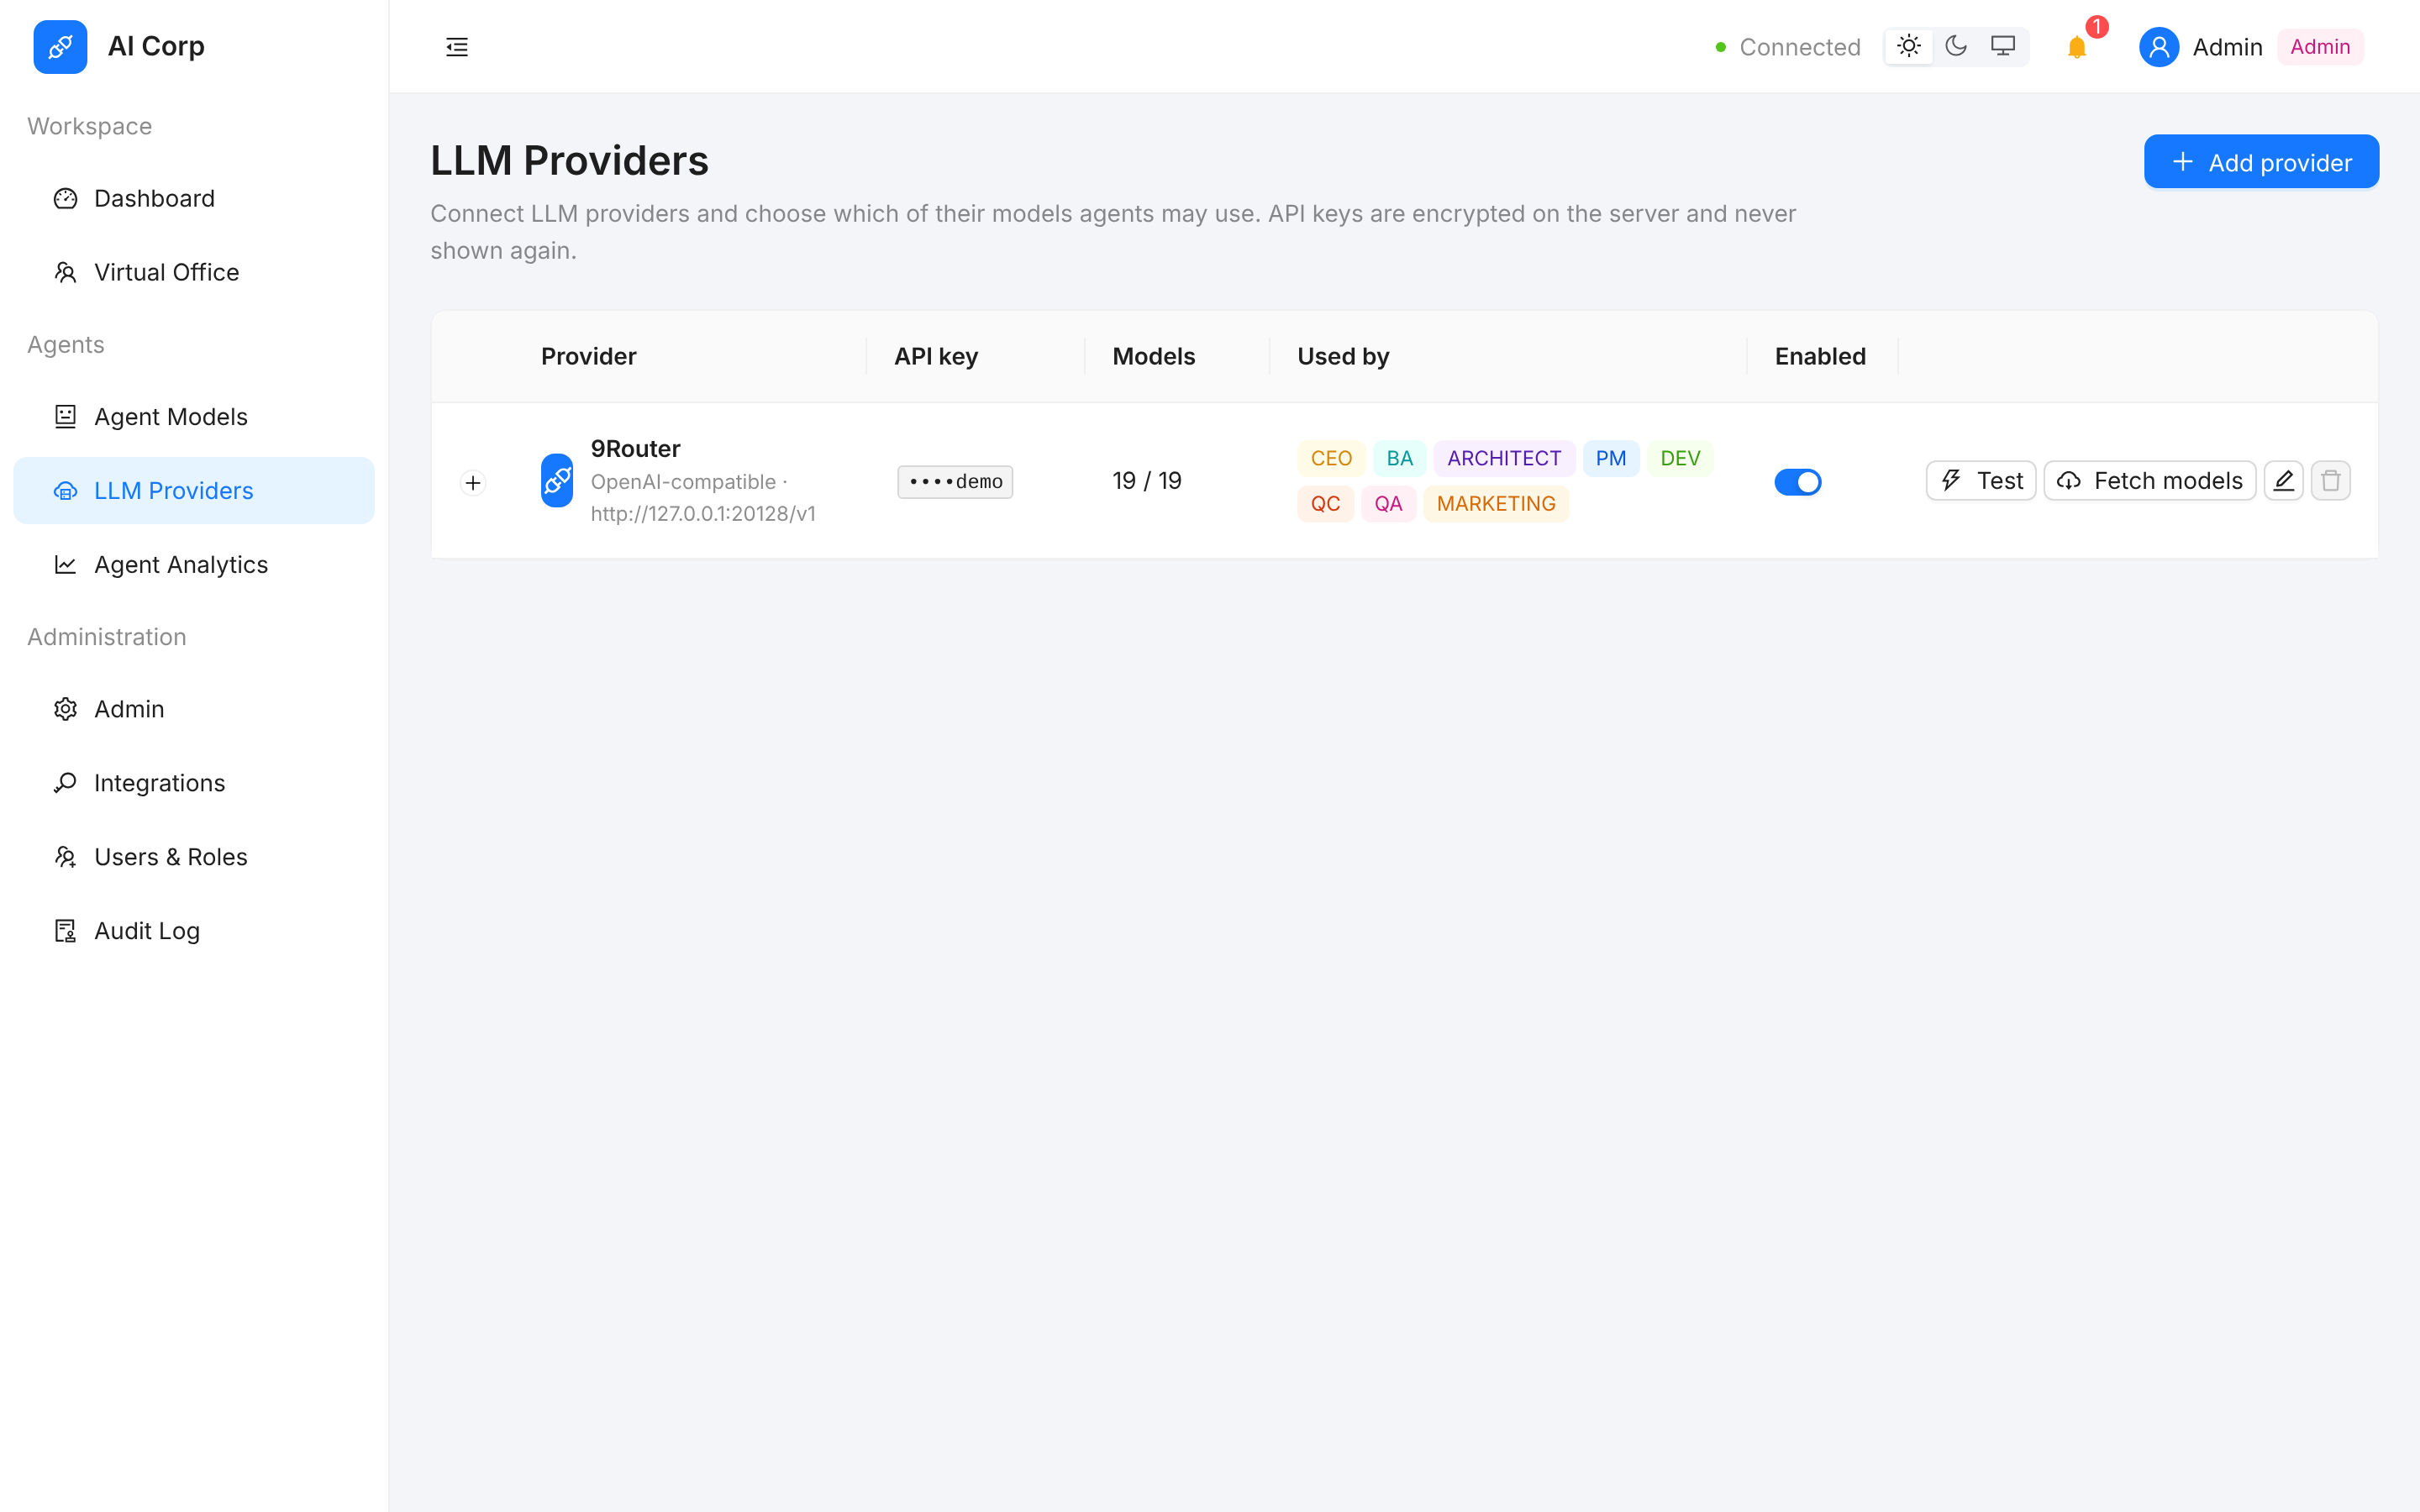
\includegraphics[width=\textwidth]{anh/providers.png}
\end{figure}

\section{Giao diện người dùng}
\label{sec:giao-dien}

Ứng dụng web viết bằng React và dùng nhãn tiếng Anh. Ở bản mới nhất, toàn bộ giao diện được chuyển sang Ant Design 6. Đợt nâng cấp này chỉ đụng tới phần hiển thị: logic, lời gọi API và tính năng giữ nguyên, và 44 kiểm thử web vẫn đạt như trước. Những thay đổi chính gồm:

\begin{itemize}
\item \textbf{Chủ đề giao diện.} \code{AppThemeProvider} gom màu sắc, cỡ chữ, bo góc vào các design token của Ant Design và xuất chúng thành biến CSS. Người dùng chọn chế độ sáng, tối hoặc theo hệ điều hành bằng ba nút ngay trên thanh đầu trang, và có thể bật chế độ gọn để bảng, biểu mẫu dày hơn. Lựa chọn được lưu trong trình duyệt qua một store Zustand. Mỗi vai trò tác tử được gán một tên màu có sẵn của Ant Design (CEO vàng, Architect tím, DEV xanh lá\ldots), và sắc độ cụ thể được chọn theo chế độ sáng hay tối.
\item \textbf{Khung trang mới.} Thanh bên chia nhóm \textit{Workspace}, \textit{Agents}, \textit{Administration}, thu gọn được về dạng biểu tượng, và chỉ hiện mục mà vai trò của người dùng được vào. Thanh đầu trang có chấm báo kết nối thời gian thực (\textit{Connected}), nút đổi chủ đề, chuông báo các phê duyệt đang chờ và menu tài khoản. Hai thành phần dùng chung \code{PageHeader} và \code{StatCard} giúp các trang có cùng một kiểu tiêu đề và thẻ số liệu.
\item \textbf{Dùng đúng thành phần cho từng việc.} Thông tin dự án và phê duyệt hiện bằng \code{Descriptions}, số liệu bằng \code{Statistic}, tiến trình và lịch sử bằng \code{Timeline} và \code{Steps}, cây tệp sản phẩm bằng \code{Tree}, khung xem tệp chia đôi bằng \code{Splitter}. Lúc đang tải thì hiện \code{Skeleton}, trang không có quyền hoặc không tồn tại thì hiện \code{Result}. Thông báo và hộp thoại đi qua \code{App.useApp()} để nhận đúng chủ đề đang dùng.
\item \textbf{Phòng họp và biểu đồ.} Khung trò chuyện của Phòng họp dựng lại bằng Ant Design X, thư viện thành phần dành cho giao diện AI, nên mỗi bước suy nghĩ của tác tử hiện thành một khối \textit{Thinking} mở ra xem được. Biểu đồ chi phí và phân tích chuyển từ Recharts sang Ant Design Charts (\code{@ant-design/plots}), dùng chung màu với chủ đề.
\item \textbf{Tải nhanh hơn.} Mỗi trang được tải lười (\code{React.lazy}) theo route, còn Vite tách React, Ant Design, Ant Design X và thư viện biểu đồ thành các gói riêng. Các gói thư viện ít đổi nên trình duyệt giữ được trong bộ đệm lâu hơn.
\end{itemize}

Các màn hình chính gồm \textit{Dashboard}, \textit{Virtual Office}, trang chi tiết dự án, \textit{Agent Models}, \textit{Agent Analytics}, \textit{LLM Providers}, \textit{Users \& Roles}, \textit{Audit Log} và \textit{Integrations}. \textit{Dashboard} liệt kê dự án, có tìm kiếm, lọc theo trạng thái, sắp xếp, và cho thấy tiến độ thật của lượt chạy cùng chi phí (Hình~\ref{fig:dashboard}). \textit{Virtual Office} hiện trạng thái tám tác tử theo thời gian thực bên cạnh Phòng họp. Trang chi tiết dự án có sáu tab: kết quả, sản phẩm, báo cáo, Kanban, mốc và lượt chạy. Tab \textit{Artifacts} gồm tóm tắt OOAD, kết quả cổng chất lượng, cây tệp, trình xem Markdown, mã nguồn, sơ đồ PlantUML do máy chủ PlantUML nội bộ render, và nút tải cả dự án về dạng zip.

\begin{figure}{Bảng điều khiển danh sách dự án ở chế độ sáng}
\label{fig:dashboard}
\centering
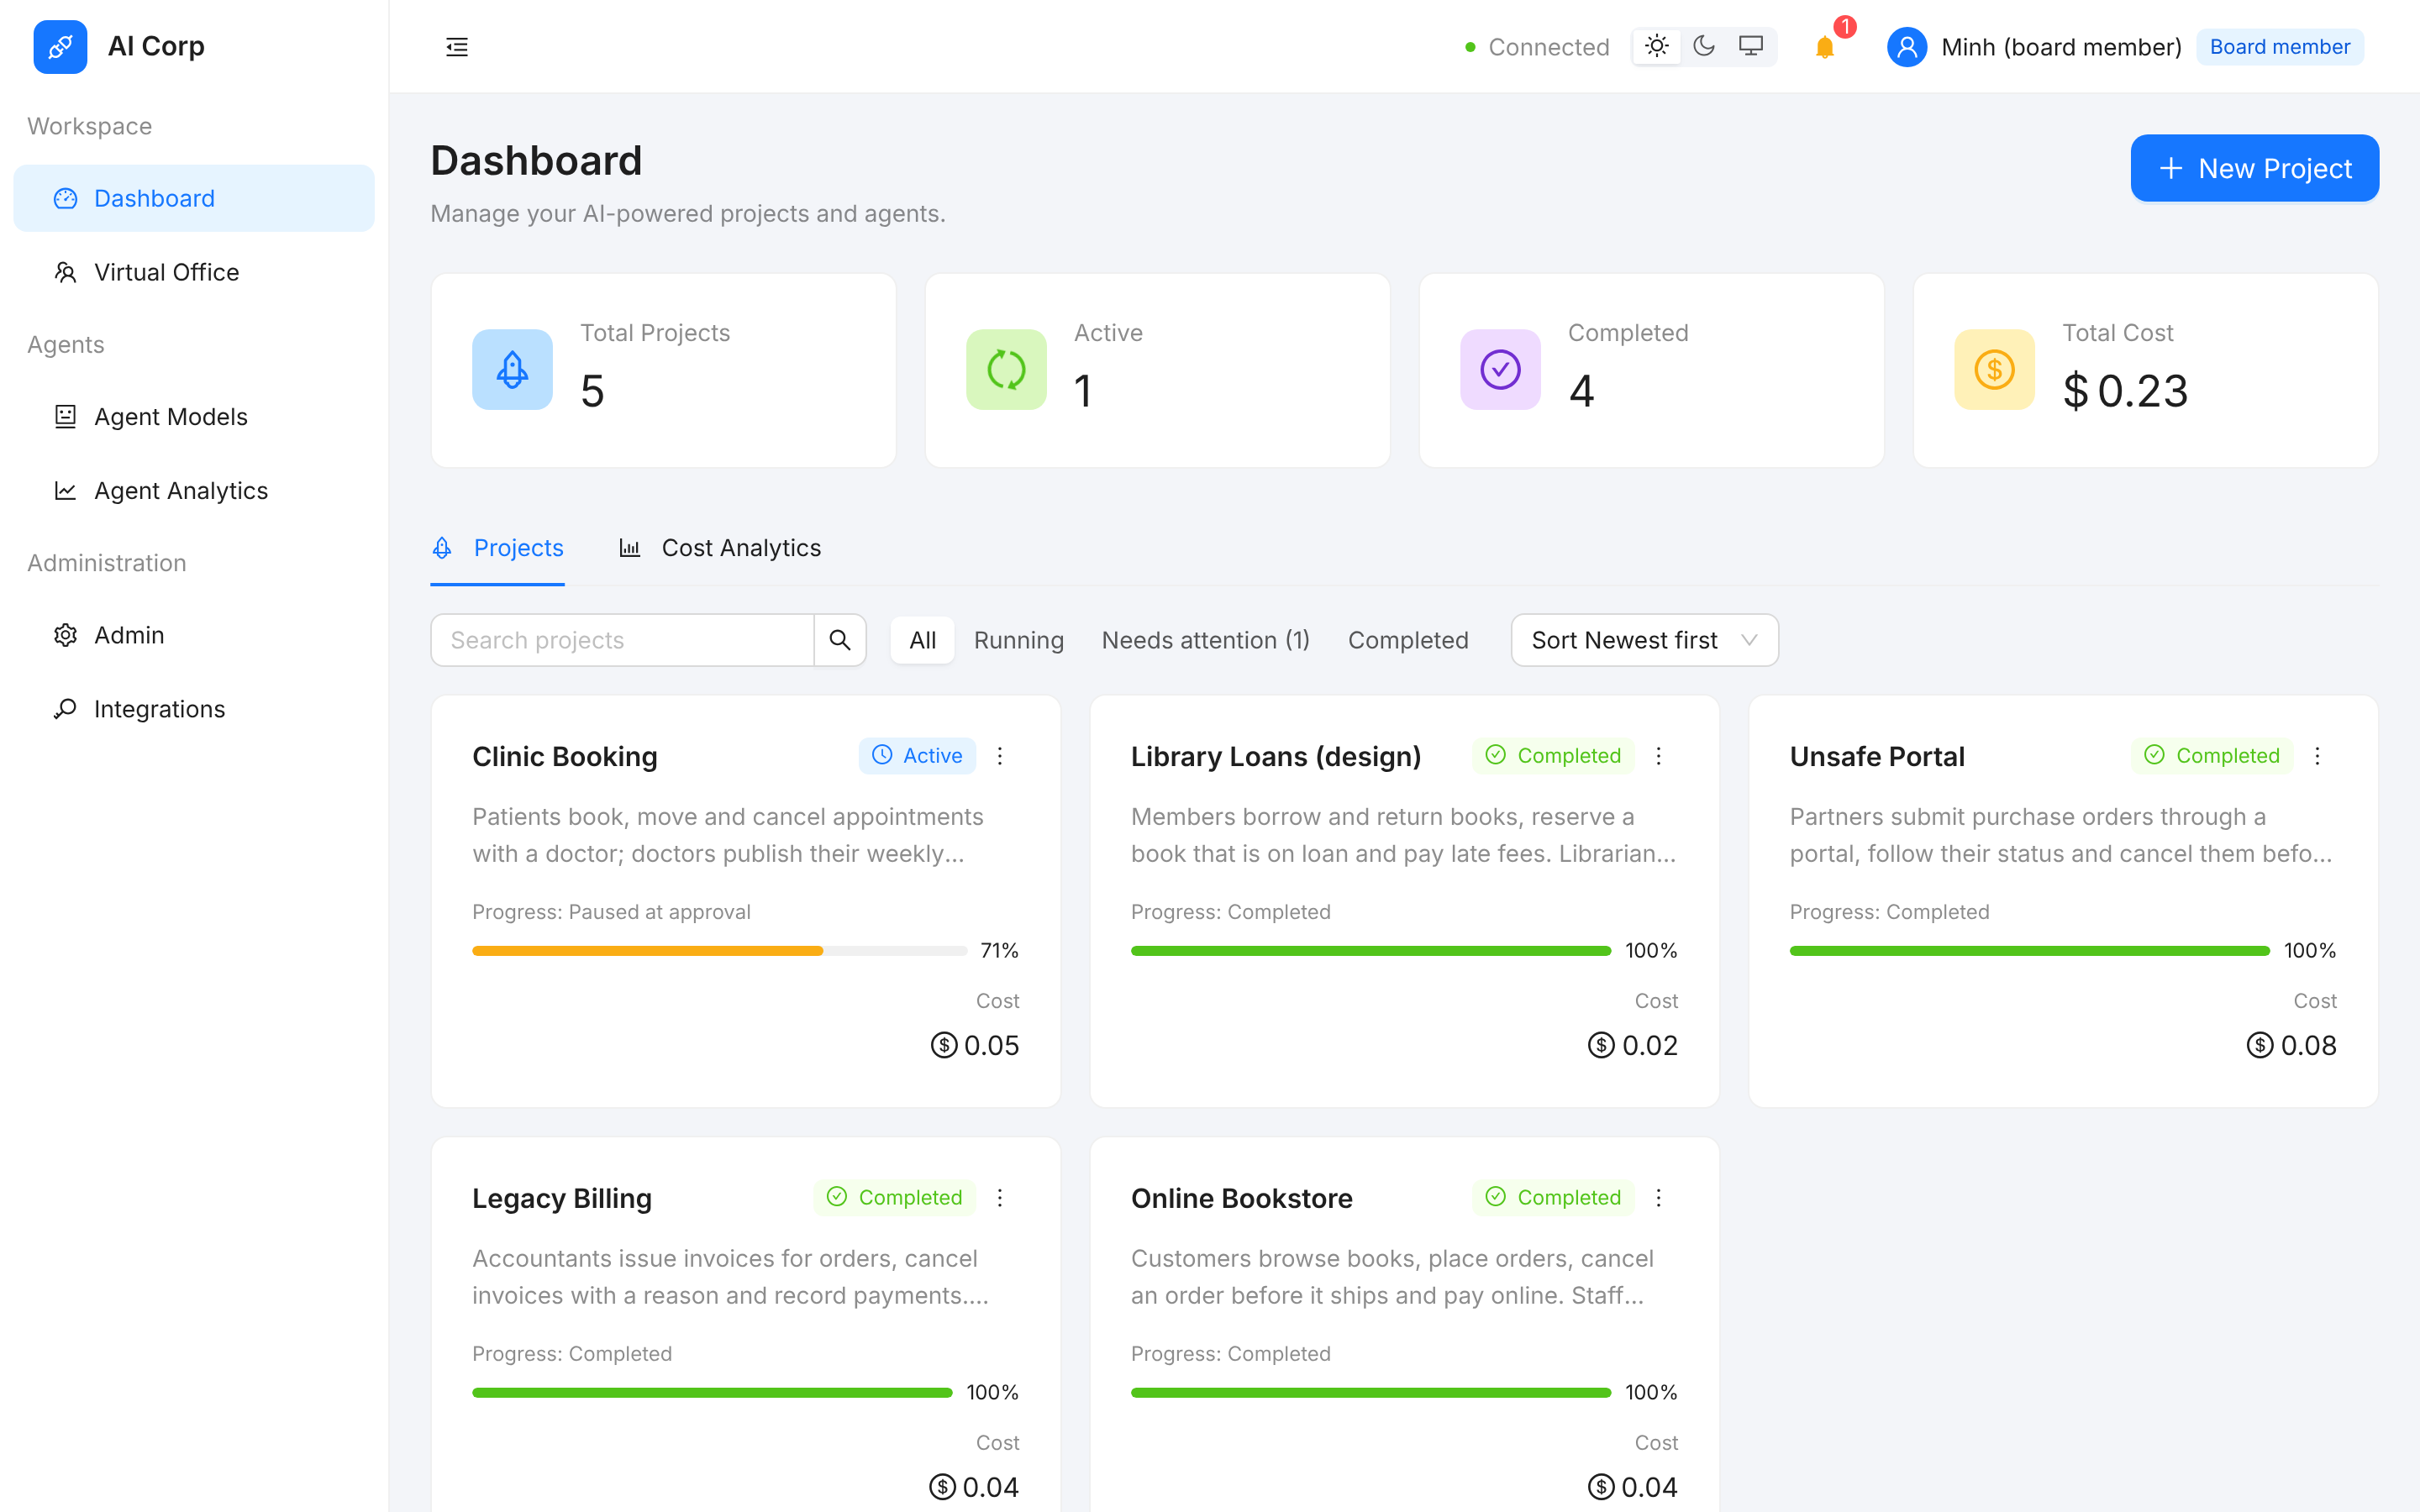
\includegraphics[width=\textwidth]{anh/dashboard.png}
\end{figure}

Hình~\ref{fig:timeline} là tab \textit{Workflow Runs} của dự án Unsafe Portal. Thanh tím là quy trình con, thanh xanh là từng bước của tác tử. Có thể thấy rõ vòng lặp: QA từ chối ở lần rà soát đầu, công việc quay lại DEV, rồi QC và QA chạy thêm một lượt. Bên dưới là danh sách ảnh chụp, mỗi ảnh có nút khôi phục, nút này chỉ bấm được khi lượt chạy đang tạm dừng hoặc đã lỗi.

\begin{figure}{Dòng thời gian và ảnh chụp của một lượt chạy quy trình}
\label{fig:timeline}
\centering
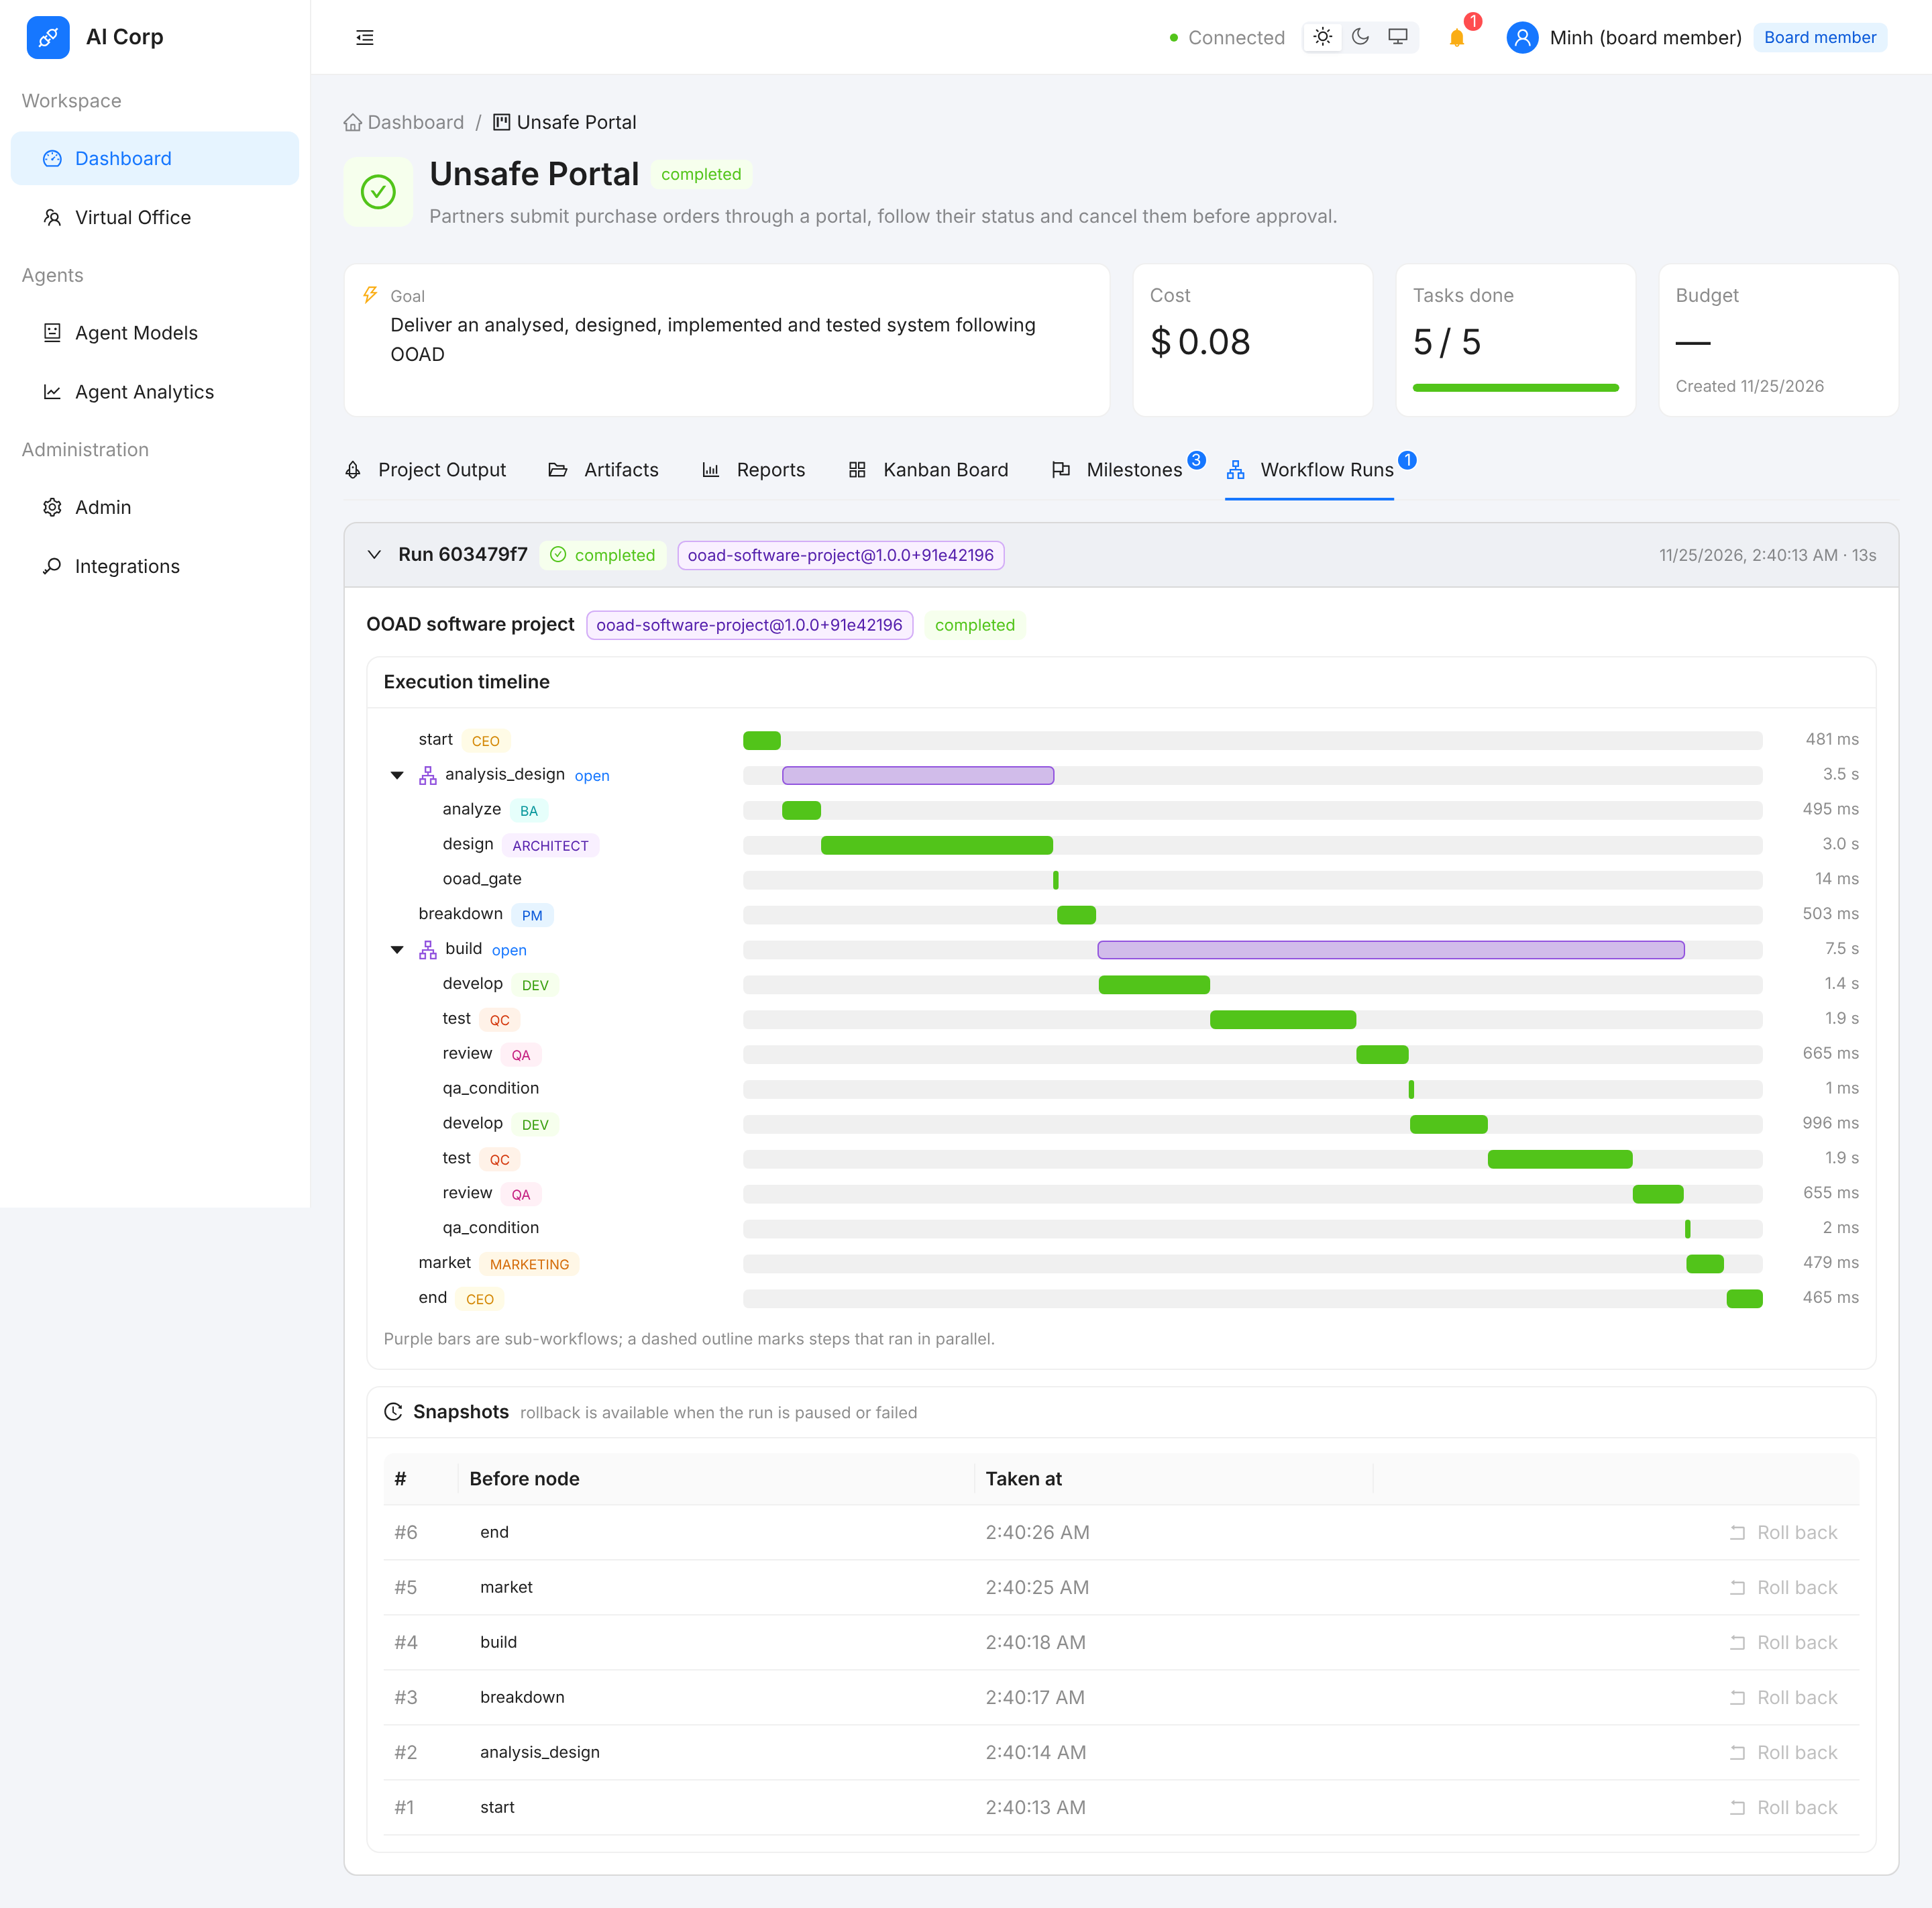
\includegraphics[width=0.85\textwidth]{anh/run-timeline.png}
\end{figure}

Khi chuẩn bị trình diễn, hai lỗi hiển thị được tìm thấy và sửa. Thẻ dự án lúc nào cũng hiện ``Starting\ldots{} 0\%'' vì dữ liệu danh sách dự án không kèm thông tin lượt chạy, còn tổng chi phí thì hiện số thực chưa làm tròn. Đợt rà soát giao diện sau đó tìm ra một lỗi nặng hơn. Trang dự án gửi yêu cầu vào phòng WebSocket với payload khác định dạng API chờ, nên sự kiện thời gian thực về công việc, quy trình và ngân sách không bao giờ tới được giao diện. Sau khi sửa, trang vào đúng phòng, tự vào lại khi mất kết nối và bỏ qua sự kiện trùng.

\section{Cấu hình triển khai}

\begin{itemize}
\item \code{apps/api/Dockerfile} có hai giai đoạn. Giai đoạn build cài phụ thuộc, sinh Prisma client, build API và script tạo dữ liệu ban đầu. Giai đoạn chạy dùng \code{tini}, chạy dưới người dùng \code{node}, có phông DejaVu cho xuất PDF và có HEALTHCHECK gọi \code{/api/health/live}. Tệp \code{docker-entrypoint.sh} chạy \code{prisma migrate deploy} rồi mới khởi động API.
\item \code{apps/web/Dockerfile} build ứng dụng với \code{VITE_API_URL=/api}, \code{VITE_WS_URL=/}, \code{VITE_PLANTUML_SERVER=/plantuml}, để mọi lời gọi đều cùng nguồn gốc qua nginx.
\item \code{docker-compose.prod.yml} và \code{.env.production.example} khai báo sáu dịch vụ (một dịch vụ chỉ chạy trong hồ sơ demo) và ba volume, chỉ công bố cổng web. Các biến môi trường mới gồm \code{LLM_SECRET_KEY}, \code{SIGNUP_ROLE}, \code{ALLOW_REGISTRATION} và \code{JWT_EXPIRATION}. Đổi \code{LLM_SECRET_KEY} thì phải nhập lại khoá của các nhà cung cấp.
\item Để cài mới từ mã nguồn, trường \code{packageManager} cố định pnpm 8.15.9, vì pnpm 8.0 lỗi trên Node 20 trở lên. Cấu hình Turborepo viết theo cú pháp của phiên bản đã cài và build gói \code{shared-types} trước. Tệp build-info của \code{shared-types} đặt trong \code{dist} để một bản clone mới luôn build ra mã.
\end{itemize}

Lúc chuẩn bị triển khai, bốn lỗi làm cấu hình cũ không chạy được đã lộ ra. Một, thư mục migration chỉ có lược đồ ban đầu, thiếu 8 bảng và nhiều cột, vì trong lúc phát triển nhóm dùng \code{prisma db push}. Hai, tệp khoá migration đặt sai chỗ. Ba, cấu hình nginx cắt mất tiền tố \code{/api}, khiến mọi lời gọi API trả 404 và WebSocket không được chuyển tiếp. Bốn, Dockerfile của API gọi điểm kiểm tra tình trạng sai đường dẫn và chạy một tệp không tồn tại. Cả bốn lỗi đều đã được sửa và kiểm chứng trong lần chạy đầu cuối triển khai ở chương sau.
